\documentclass[11pt]{article}
\usepackage{url}
\usepackage{graphicx}
\usepackage{xcolor}
\usepackage[round,sort]{natbib}
\usepackage{amsmath}
\usepackage{soul}
\usepackage{amssymb}
\usepackage{listings}
\usepackage{longtable}
\def\UrlFont{\rmfamily}
\usepackage{verbatim}
\usepackage{subfigure}
\usepackage{hyperref}
\usepackage[margin=1in]{geometry}
\usepackage{titlesec} 
\titleformat{\section}[runin]
  {\normalfont\large\bfseries}{\thesection}{1em}{}
\titleformat{\subsection}[runin]
  {\normalfont\small\bfseries}{\thesubsection}{1em}{}

\hypersetup{colorlinks=true,linkcolor=black,urlcolor=blue,citecolor=black}
\newcommand{\code}{\texttt}

\renewenvironment{abstract}
               {\list{}{\rightmargin\leftmargin}%
                \item[\hspace{10mm}\textbf{Abstract --- }]\relax}
               {\endlist}

\begin{document}

%\mainmatter
\title{Bayesian Hierarchical Time Series on NFL Home-Game Attendance}
\author{Cason Wight -- December 5, 2020}
\date{\vspace{-5ex}}
\maketitle


\begin{abstract}
The NFL is a multi-billion dollar franchise; however, due to the Covid-19 pandemic, its revenue is taking a hit, especially on ticket sales. This project uses a simple Bayesian hierarchical times series to model the weekly average home game attendance for $31$ teams. Team-specific intercepts and $\text{lag}(1)$ attendance effects were used, with a hyperprior on the center of these parameters. An effect of previous year's wins was also included, along with an overall error term. Three different priors and two different computational approaches were used on this model. Based on the prior used, between $0$ and $14$ teams' previous year's attendance has an insignificant effect on attendance. Also, all modeling approaches agree that an additional win increases the following year's weekly attendance by roughly $300$. Upon comparing the predicted 2020 attendance with the observed weekly average attendance, it was found that the NFL is likely to lose $\$2.1$ bil. in ticket sales in 2020.
\end{abstract}

\vspace*{-.5\baselineskip}
\section{Introduction}

%\subsection{About}

Covid-19 has had a major impact on many areas, sports being one of the foremost affected. Recently, \cite{ehrlich2020covid} estimated that for the NFL, MLB, NBA and NHL, Covid-related losses on gate tickets alone are 6.8 billion USD. Attendance at football games this year is certainly an anomaly, but fan attendance always varies across years and teams. Last year, roughly $15\%$ of the NFL's revenue came from ticket sales alone, making about $\$2.3$ bil. in 2019. 

As such a large revenue source, many have modeled attendance at these games. \cite{welki1999us} found that games with better teams, teams of a similar level, good weather, and low price typically have higher attendance. \cite{coates2010week} show some evidence that home-game attendance is slightly higher in games where the home team is expected to win and much more evidence that home-game attendance is low in games where the home team is expected to lose.  We will explore how previous year's attendance and previous year's number of games won can affect the home-game attendance of a team.

\vspace*{-.5\baselineskip}
\subsection{Data}

The data used in this project are obtained from the \href{https://github.com/rfordatascience/tidytuesday/blob/master/data/2020/2020-02-04}{Tidy Tuesday Project}, a repository of the \href{https://www.rfordatasci.com/}{R for Data Science Online Learning Community}. This site posts weekly data sets for educational purposes. The NFL Attendance data set contains information on attendance, team standings, and the games themselves. There are many covariates that could be interesting to consider in predicting a team's yearly average home-game attendance, but this project will focus only on the previous year's average home-game attendance and the previous year's number of wins for each team. This project uses $31$ teams for which 2000-2019 home-game attendance data is available. There are 16 regular season games for each of these teams each season.

The team with the most wins during this time period is the New England Patriots. They won 232 of 304 regular-season games. The Cleveland Browns had the fewest number of wins (96 of 304). Figure \ref{fig:games_won} shows some of the 31 teams and their winning rate since 2000. Ultimately, this project is interested in home-game weekly average attendance each year. The team with the highest average home-game attendance is the Washington (formerly Redskins) football team. The team with the lowest is the Las Vegas Raiders. Yearly average attendance for different teams is shown in Figure \ref{fig:year_att}, Some teams (like the Patriots or Packers) have stadiums that are regularly at capacity. Other teams (like the Jaguars or Buccaneers) have many more seats than are typically filled, so attendance is more volatile. Incorporating stadium capacity would be an interesting modeling technique, but is too complex for this project.

\begin{figure}
    \centering
    \begin{minipage}{.475\textwidth}
        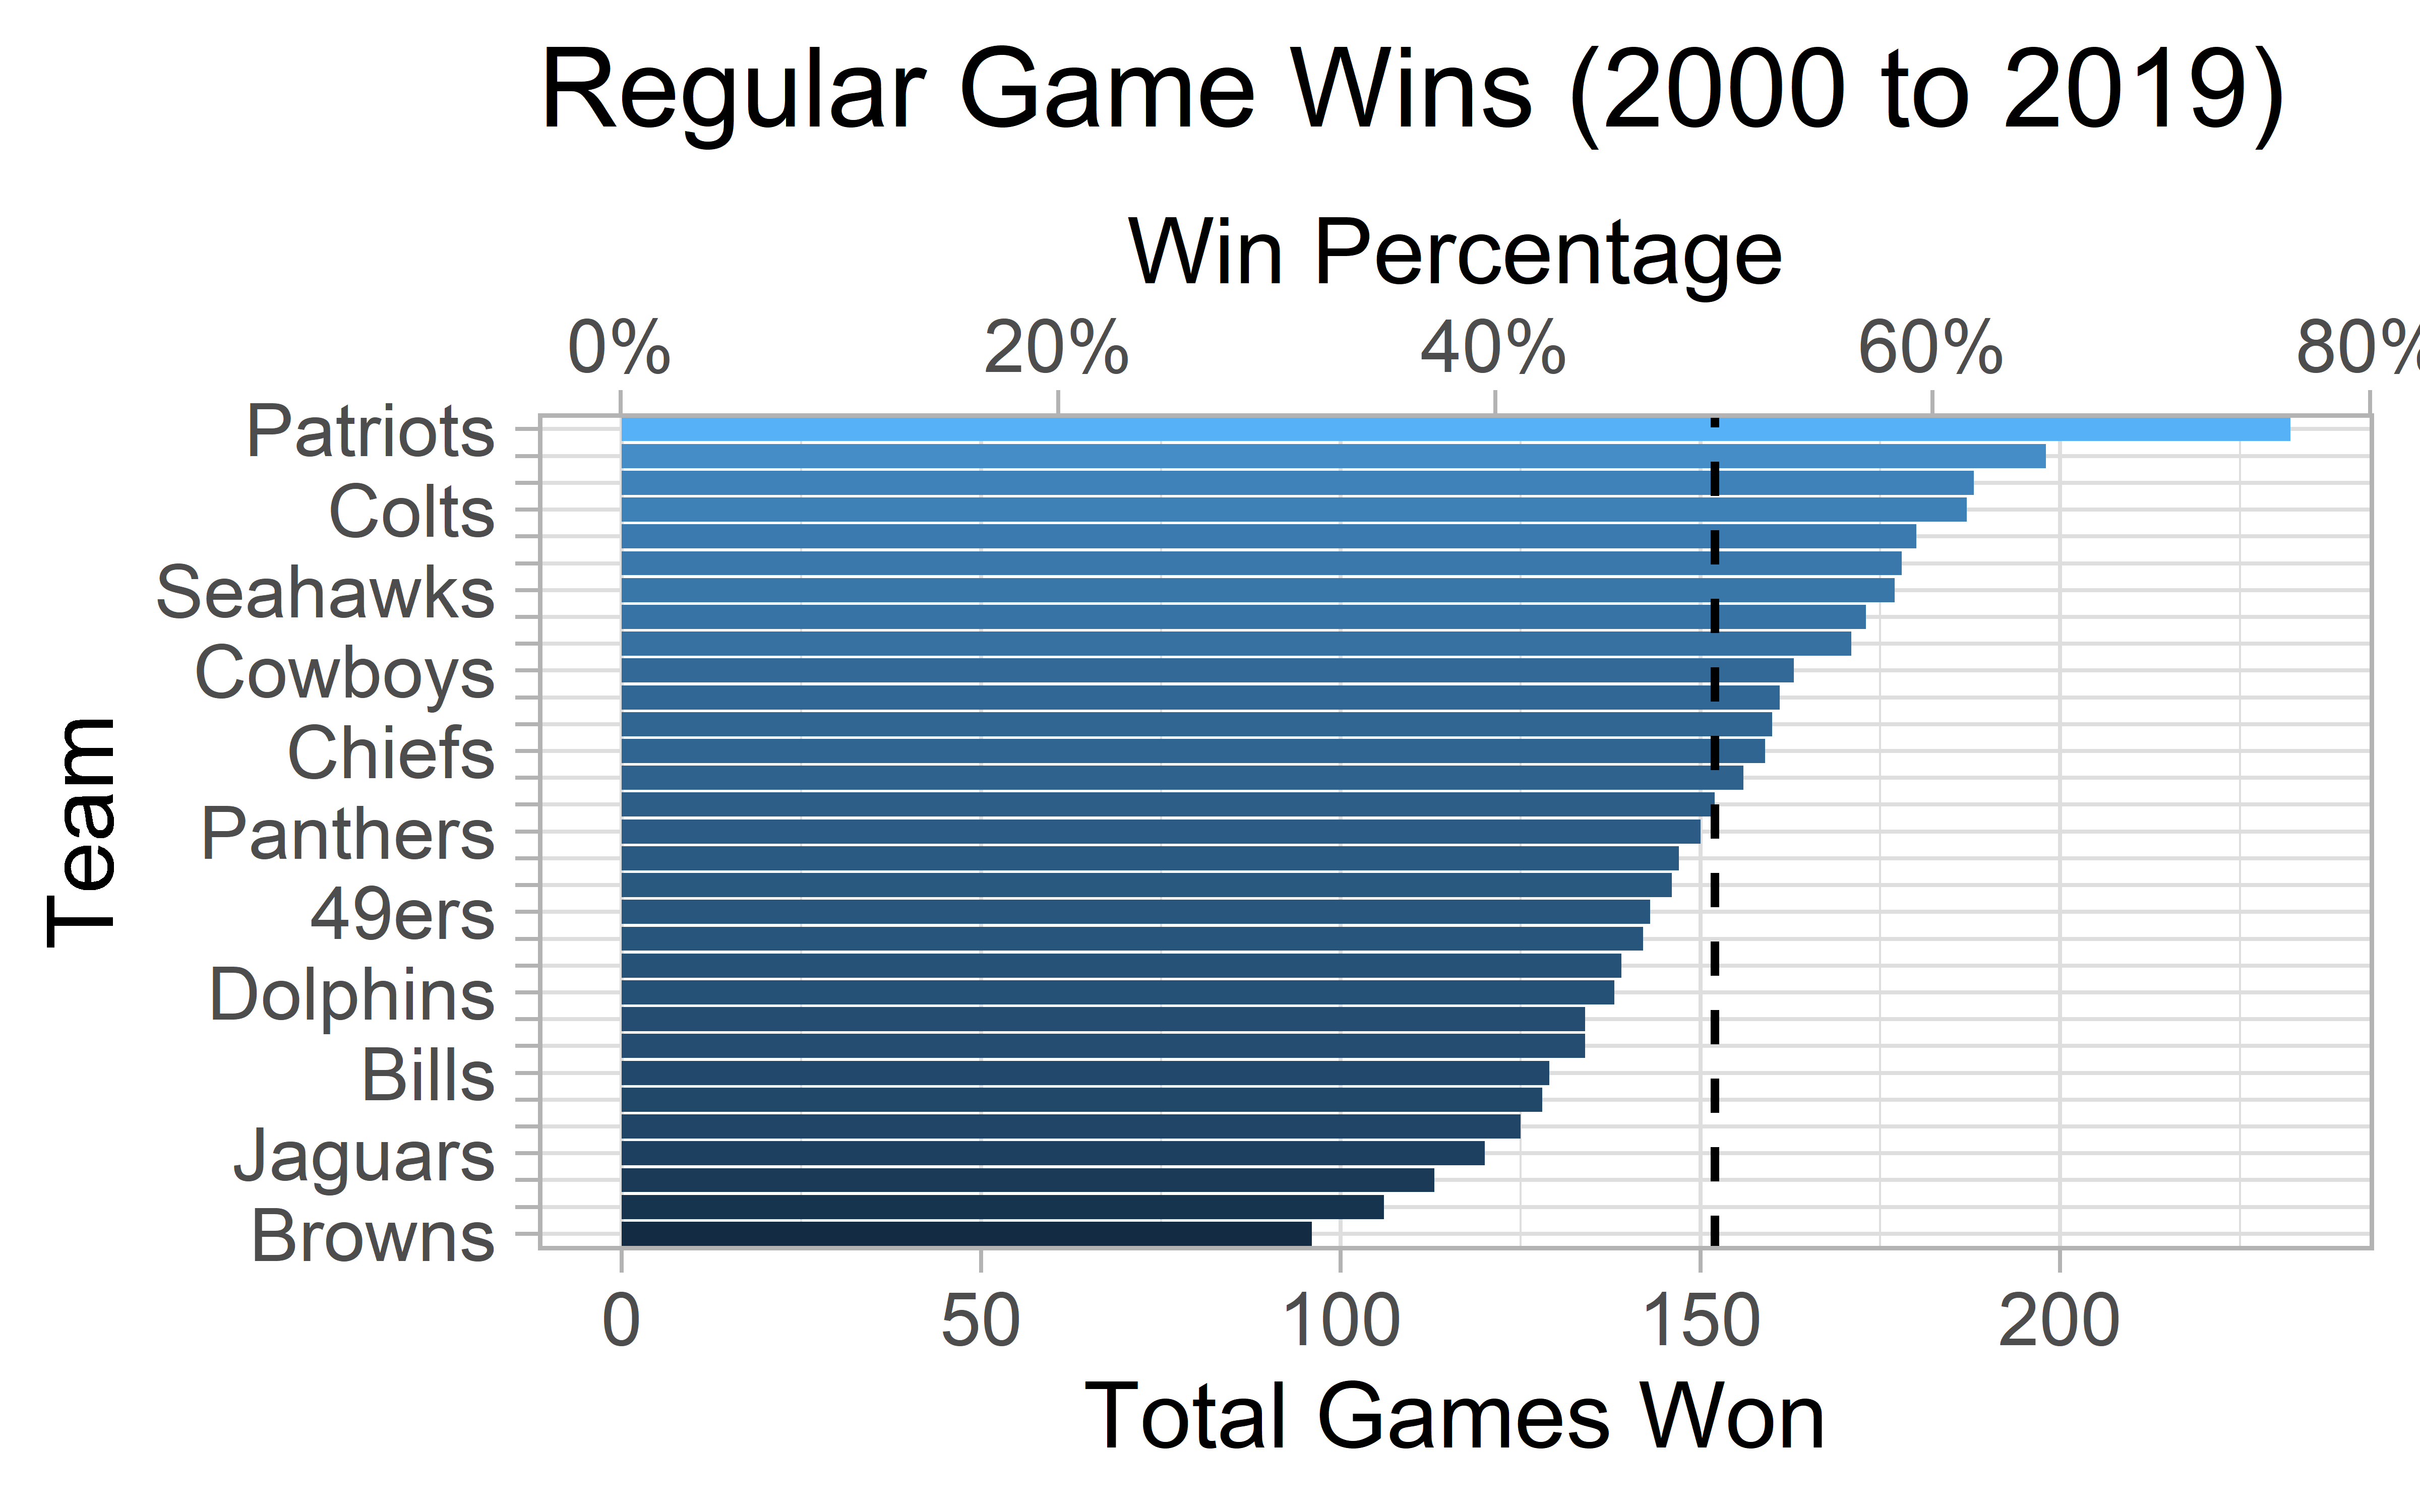
\includegraphics[width=\linewidth]{Games_Won.png}
        \caption{\footnotesize Regular-season wins by each team. Games include those from 2000 to 2019. Only some team names are shown here. The dashed line represents $50\%$ regular-season win rate. \vspace*{-.5\baselineskip}}
        \label{fig:games_won}
    \end{minipage}\hfill
    \begin{minipage}{.475\textwidth}
        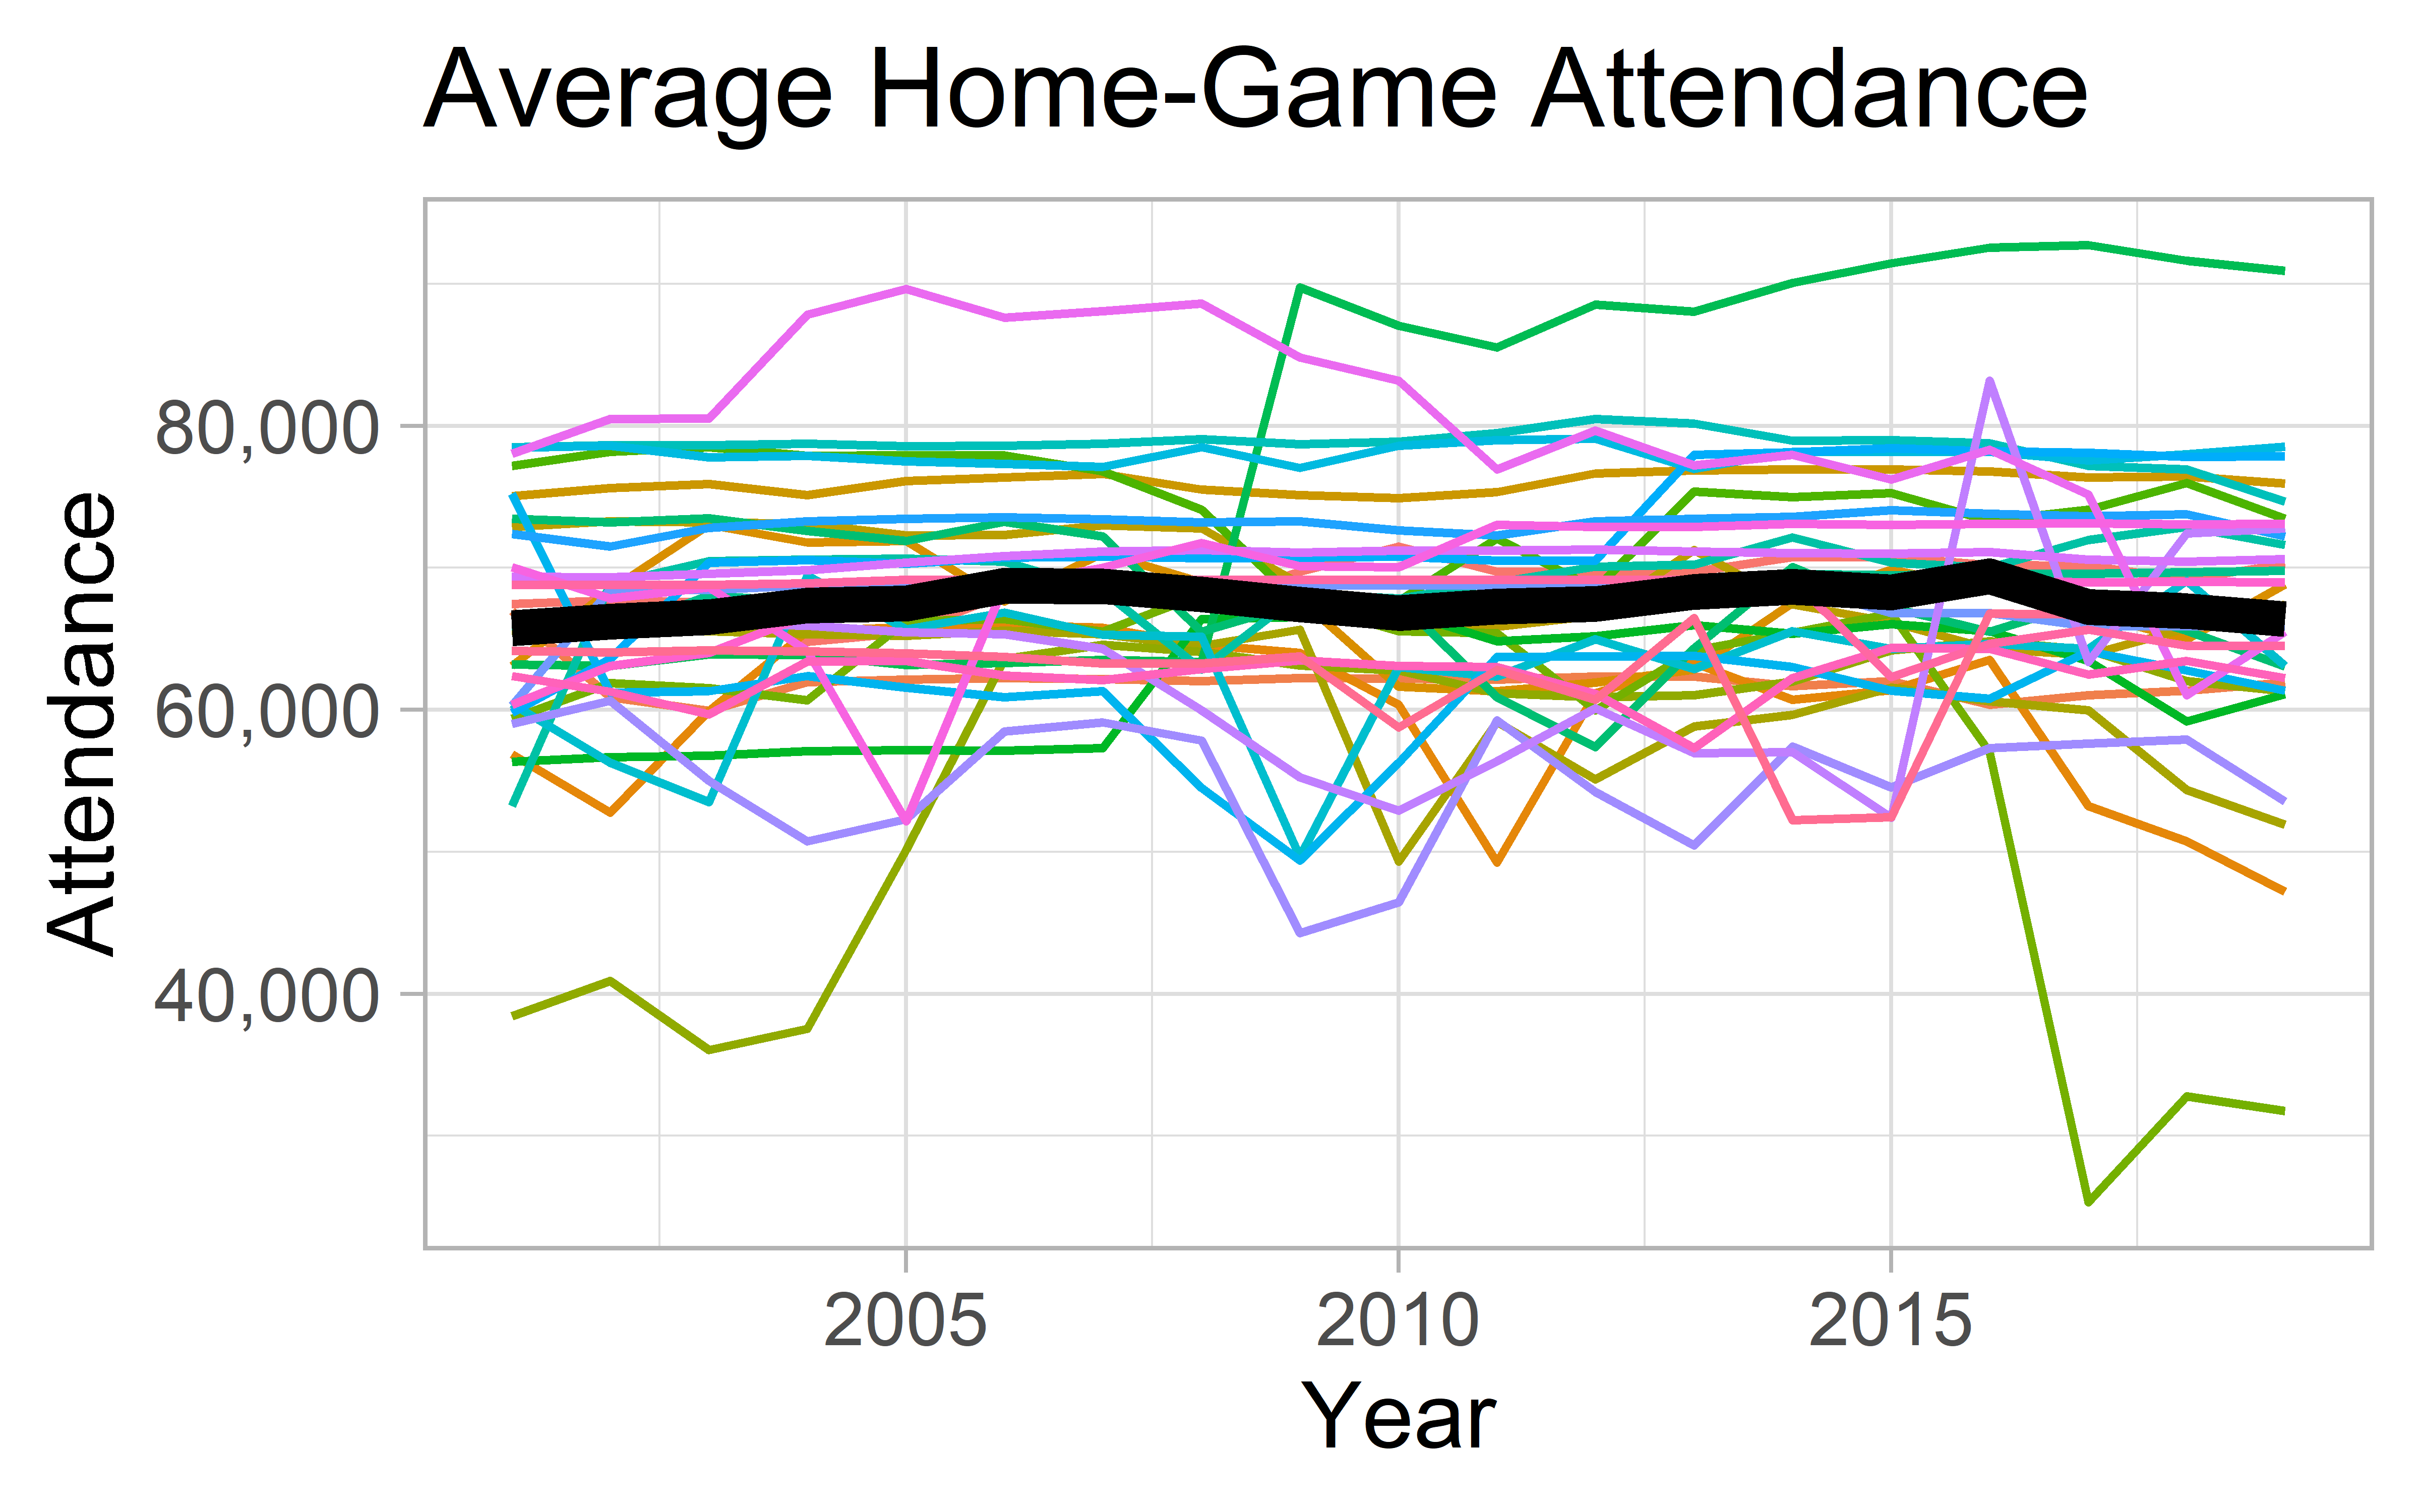
\includegraphics[width=\linewidth]{Yearly_Attendance.png}
        \caption{\footnotesize Weekly average attendance per year. The different colors each represent one of the $31$ included teams. The solid black line is the overall average attendance. \vspace*{-.5\baselineskip}}
        \label{fig:year_att}
    \end{minipage}
\end{figure}

\vspace*{-.5\baselineskip}
\subsection{Goals}

This project implements a Bayesian time series analysis on NFL average attendance data during the years 2000 to 2019. This analysis will be hierarchical, with certain parameters for each team drawn from hyper-prior distributions. The goals of this project include the following:
\begin{enumerate}
    \item Develop a Bayesian time series analysis method, with a single covariate, and test the model with a simulation study
    \item Estimate the average yearly change in attendance and $\text{lag}(1)$ effect of attendance for each team, estimate the impact of previous year's number of wins on attendance across all teams, predict would-be attendance for 2020, and stress-test these results with various prior selections
    \item Perform an equivalent analysis under a Frequentist paradigm (linear regression with lag(1) coefficient) and compare the two 
\end{enumerate}

\vspace*{-.5\baselineskip}
\subsection{Model}

Based on the goals and data available, the model should include team-specific intercept parameters, $\alpha_i$s, and $\text{lag}(1)$ team-specific regression parameters, $\beta_{i}$s. These parameters will have hyper-prior distributions, so the posterior distributions will differ between teams, but there will be a sharing of strength in determining the overall intercept and coefficient. Intuitively, the $\alpha_i$ term is the baseline level of attendance for a team $i$, and $\beta_i$ is the additive effect of the previous year's average home game attendance for team $i$. Additionally, a $\theta$ term in the model will report the additive effect of the previous year's number of wins on attendance; this term will not be team specific. Finally, $\sigma$ is the standard deviation of the remaining error from this model and will not be team specific either. 

This model and the research questions of the project could assist the NFL to understand which teams have the most reliance on previous year's attendance. The NFL could also understand how robust attendance is from one year to the next and how wins affect the teams' fan attendance. Additionally, the NFL is likely interested in how much revenue they have lost in 2020 from having reduced attendance due to Covid-19. The predicted would-be attendance is a good place to start with this type of question.

\vspace*{-.5\baselineskip}
\section{Methodology}

%\subsection{Model Details}

As stated, the model used in this project will measure the effect of previous year's attendance and previous year's number of wins on current year's average home-game attendance. Each team will share in strength for the intercept and slope (effect of previous attendance), but will each have distinct parameter estimates. The effect of prior year's number of wins will be estimated simply across all teams. Thus the following model will be implemented:
\begin{align}\label{eq:model}
\begin{split}
y_{i,t}|\alpha_i,\beta_i,y_{i,t-1},\theta,x_{i,t},\sigma&\sim\mathcal{N}\left(\alpha_i+{\beta_i} * y_{i,t-1} +\theta * x_{i,t},\sigma^2\right) \\
\alpha_i|\alpha&\sim\mathcal{N}(\alpha,\lambda^2),\qquad\alpha\sim \mathcal{N}(\mu_\alpha, \sigma_\alpha^2) \\
\beta_i|\beta&\sim\mathcal{N}(\beta,\eta^2),\qquad\beta\sim \mathcal{N}(\mu_\beta,\sigma_\beta^2) \\
\theta&\sim\mathcal{N}(\mu_\theta,\sigma_\theta^2)\\
\sigma&\sim\text{Gamma}(\alpha_\sigma, \beta_\sigma)
\end{split}
\end{align}

The fixed parameters for the prior distribution include those for $\theta$, $\mu_\theta$ and $\sigma_\theta$; those for $\sigma$, $\alpha_\sigma$ and $\beta_\sigma$; those for the hyperprior $\alpha$, $\mu_\alpha$ and $\sigma_\alpha$; those for the hyperprior $\beta$, $\mu_\beta$ and  $\sigma_\beta$; the standard deviation of the $\alpha_i$s for each team, $\lambda$; and the standard deviation of the $\beta_i$s for each team, $\eta$. The marginal posterior distributions of interest are those for $\theta$, $\sigma$, $\alpha$, $\beta$, the individual $\alpha_i$s, and the individual $\beta_i$s.

%\subsubsection{Model Structure}

As shown by the flowchart in Figure \ref{fig:flowchart}, the variable parameters $\alpha$ and $\beta$ flow into each of the $\alpha_i$s and $\beta_i$s as the center of the distributions of these variable parameters. Thus, this is a hierarchical model. The relationship of each $\beta_i$ to the attendance $y_{i,t}$ of team $i$ at year $t$ is through the prior year attendance $y_{i,t-1}$, making it a $\text{lag}(1)$ effect and making the problem itself a simple time series model. The $\theta$ term is also a regression coefficient, and is connected to all $y_{i,t}$ through the prior year's number of games won $x_{i,t}$.

\begin{figure}
    \centering
    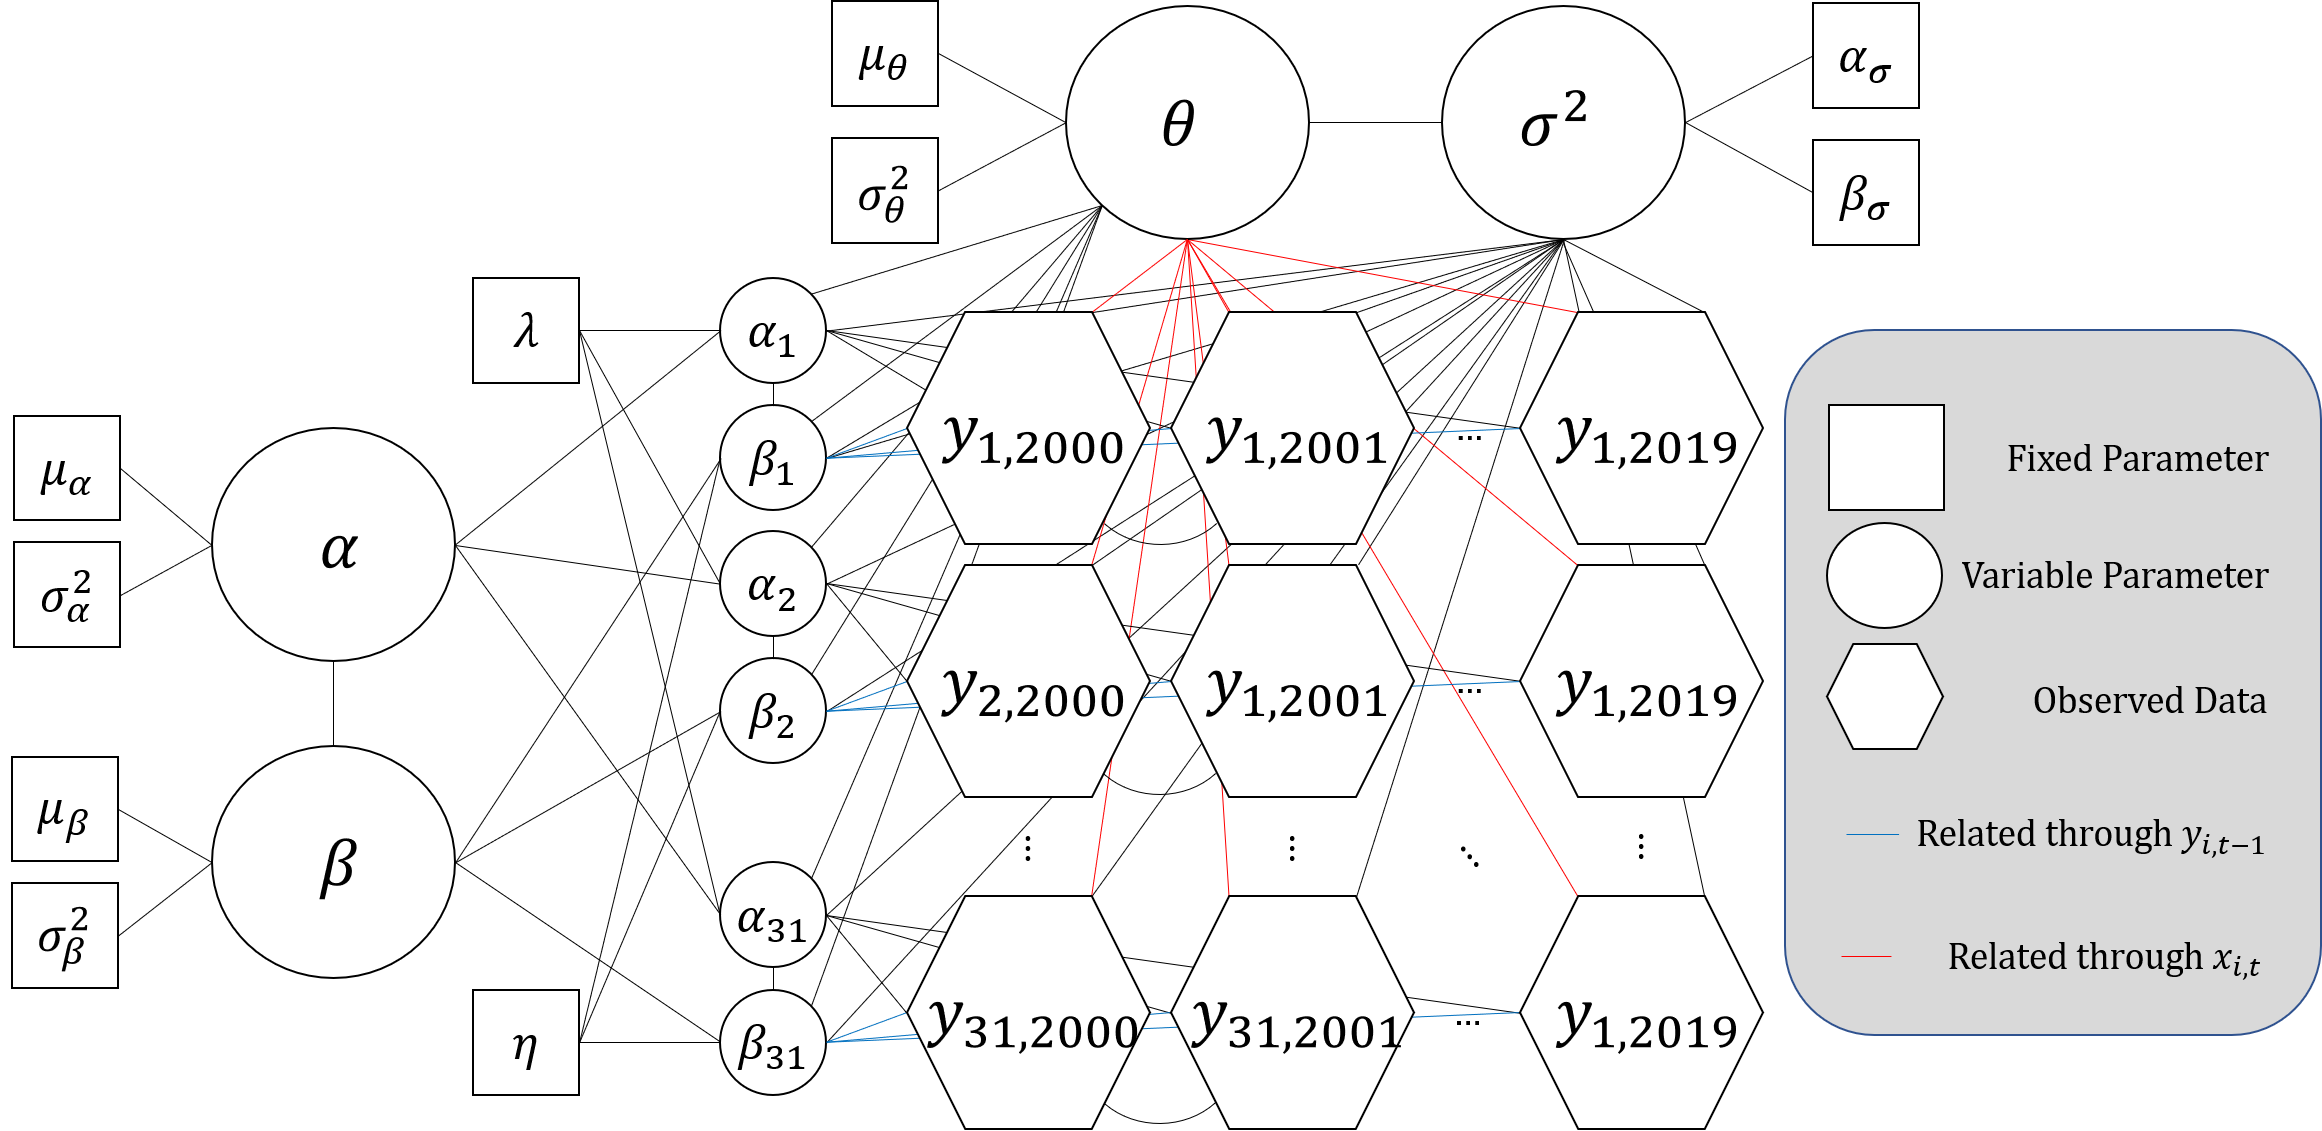
\includegraphics[width=.7\textwidth]{flowchart.png}
    \caption{\footnotesize Flowchart of Bayesian Model \vspace*{-.5\baselineskip}}
    \label{fig:flowchart}
\end{figure}

\vspace*{-.5\baselineskip}
\subsection{Prior Selection}

In this project, sensitivity analysis was performed by using three distinct sets of priors. The first prior was designed to be relatively stringent. The second had non-informative priors. The third was a compromise between the other two, being stringent in overall effects and loose in team-specific effects. Table \ref{tab:priors} shows the exact values for these priors. The general reasoning is as follows: The average NFL attendance is around $66{,}000$; the overall intercept term is likely less than this, but not by much. The best guess is that attendance from a previous year has an effect of about $.7$, which would put the intercept lower than half of $66{,}000$. For the second set of priors, the standard deviation of $\alpha$ is extremely large. For the third, this project tested more stringent overall terms (so the variance is small). The second set of priors had a center of $0$ and a large variance for the attendance effect term. The third had a center of $.6$ and a standard deviation of $.2$. In the team specific terms, the first prior had small variances, the second extremely large, and the third a compromise between the other two. the best guess is that the effect of wins would be around $1{,}000$. Due to the uncertainty, it has a standard deviation of $1{,}000$. The second prior had a much larger variance (with a center of $0$), and the third a smaller variance of $500^2$ with a center of $500$). The gamma-distributed error standard deviation, $\sigma$ was estimated to have a mean of $10{,}000$, $5{,}000$, and $5{,}000$ for the three respective priors (with corresponding standard deviations of $15{,}000$, $100{,}000$, and $1{,}000$). 


\begin{table}[ht]
    \centering
    \footnotesize
    \begin{tabular}{llccc}
         Fixed  Parameter & Interpretation & Prior 1 & Prior 2 & Prior 3 \\
         \hline
         $\mu_\alpha$ & Center of overall attendance intercept & $30{,}000$ &  $66{,}000$ & $66{,}000$ \\
         $\sigma_\alpha$ & Std. deviation of overall attendance intercept & $20{,}000$ &  $2{,}000{,}000$ & $6{,}000$ \\
         $\lambda$ & Std. deviation of team attendance intercepts & $8{,}000$ &  $100{,}000$ & $15{,}000$ \\
         $\mu_\beta$ & Center of overall attendance effect & $.7$ &  $0$ & $.6$ \\
         $\sigma_\beta$ & Std. deviation of overall attendance effect & $.5$ &  $2{,}000{,}000$ & $.2$ \\
         $\eta$ & Std. deviation of team attendance effects & $.1$ &  $20$ & $.4$ \\
         $\mu_\theta$ & Center of wins effect & $1{,}000$ &  $0$ & $1{,}000$ \\
         $\sigma_\theta$ & Std. deviation of wins effect & $1{,}000$ &  $2{,}000{,}000$ & $500$ \\
         $\alpha_\sigma$ & Shape of error in model: $\frac{\text{mean}^2}{\text{variance}}$ & $\left(\frac{10{,}000}{15{,}000}\right)^2$ &  $\left(\frac{5{,}000}{100{,}000}\right)^2$ & $\left(\frac{5{,}000}{1{,}000}\right)^2$ \\
         $\beta_\sigma$ & Rate of error in model: $\frac{\text{mean}}{\text{variance}}$ & $\frac{10{,}000}{15{,}000^2}$ &  $\frac{5{,}000}{100{,}000^2}$ & $\frac{5{,}000}{1{,}000^2}$ \\
         \hline
    \end{tabular}
    \caption{\footnotesize Priors selected for modeling. The first prior is relatively informative. The second is non-informative. The third is more informative for overall parameters, but non-informative for team-specific parameters. \vspace*{-.5\baselineskip}}
    \label{tab:priors}
\end{table}

\vspace*{-.5\baselineskip}
\subsection{Computational Approach}

Two different sampling methodologies were applied to these data to sample from the model specified in Equation \ref{eq:model}. The first approach is obtaining Markov-Chain Monte Carlo (MCMC) samples through the Metropolis algorithm, implemented ``by hand" in \code{R}. A simple definition of the Metropolis algorithm is given here, but see \cite{bhanot1988metropolis} for a more thorough introduction. The Metropolis algorithm is a method of obtaining samples from a posterior distribution, given its unnormalized posterior density function. The algorithm is as follows:

\begin{enumerate}
    \item Start with an initial sample $\boldsymbol{\psi}_0$ for the parameters (arbitrary, but hopefully reasonable).
    \item For samples $i=\{1,\dots,B\}$, do the following:
    \begin{itemize}
        \item Propose a set of parameters $\boldsymbol{\psi}^*$ from a proposal distribution $g(\boldsymbol{\psi}^*|\boldsymbol{\psi}_{i-1})$. constrained by $g(\boldsymbol{\psi}_a|\boldsymbol{\psi}_b)=g(\boldsymbol{\psi}_b|\boldsymbol{\psi}_a)$.
        \item Compute the Metropolis ratio $r_{\text{H}}=\frac{p(\boldsymbol{\psi}^*)}{p(\boldsymbol{\psi}_{i-1})}$, where $p(\cdot)$ is the unnormalized joint posterior distribution.
        \item With probability $\min{1,r_{\text{H}}}$, set $\boldsymbol{\psi}_i=\boldsymbol{\psi}^*$; otherwise set $\boldsymbol{\psi}_i=\boldsymbol{\psi}_{i-1}$
    \end{itemize}
\end{enumerate}

This algorithm results in $B$ correlated posterior samples. The proposal distribution is tuned until roughly $40\%$ of samples are accepted. Additionally, a burn in and thinning are also required for optimal sampling. This projects implements the Metropolis algorithm in \code{R}, with a burn in of $5{,}000$ samples, thinning to every $25^{\text{th}}$ sample. Obtaining a single chain of $20{,}000$ samples took nearly $15$ hours using a single core. The proposal distribution for these samples was a multivariate normal distribution, centered on the parameter samples from the previous Metropolis iteration. The correlations between variables in the proposal was $0$ (which could be adjusted for improved sampling in the future). The variances were adjusted until a reasonable acceptance rate was achieved. The acceptance rate for the samples was $49\%$, which is close enough to the target of $40\%$. 


The second approach is Hamiltonian MCMC, applied through \code{stan}. \code{stan} is an out-of-the-box software that compiles Bayesian models in C++, making sampling very quick. This software interfaces easily with \code{R}. Hamiltonian MCMC is a form of the Metropolis-Hastings algorithm with high acceptance probabilities. Essentially, Hamiltonian MCMC uses a proposal distribution that corresponds to the calculated posterior density, so the $r_{\text{H}}$ ratio is typically high, and samples are not very correlated. Because so few samples get rejected, less thinning is necessary, samples often converge faster, and thus samples can be superior to other methods. In this project, the samples from \code{stan} had much better convergence and autocorrelation diagnostics then the samples obtained by hand. Additionally, the sampling is much faster, so $4$ chains were obtained, rather than a single chain for each parameter. Four chains, totaling $36{,}000$ samples (with a burn in of $1{,}000$ and thinning by every other sample) took just over an hour, using four cores. Because sampling using \code{stan} appears superior, it was used for all three priors. The by-hand sampling was done only on the first prior and compared to the \code{stan} samples to show agreement. 

\vspace*{-.5\baselineskip}
\subsection{Model Checking}\label{sec:diag}

%\subsubsection{Computational Diagnostics}

Several different computational diagnostics are available for checking the validity of posterior MCMC samples. This project uses trace plots, autocorrelation (ACF) plots, effective sample sizes, and the Gelman statistic $\hat{R}$. Each of these diagnostics can reveal various potential problems in sampling, but non can completely absolve the samples of issues. 

Trace plots simply take each parameter of the posterior samples and show the change in the parameter estimate at each step of the sampling process. Trace plots that don't reveal any problems will have random noise within the reasonable bounds of the posterior distribution. The \code{stan} samples resulted in a trace plot of this type. The by-hand samples have much worse diagnostic results. Typically, more samples, more thinning, and/or more burn in could help resolve problems identified by a trace plot. Figure \ref{fig:diagnostics} shows that the stan samples have random noise, while the by-hand samples are correlated and convergence is unsure. The plot here is just for the $\alpha$ samples under the first prior, but the trace plots look nearly identical for all \code{stan} samples. The by-hand samples show similar problems for the remaining parameters as well.

\begin{figure}[ht]
    \centering
    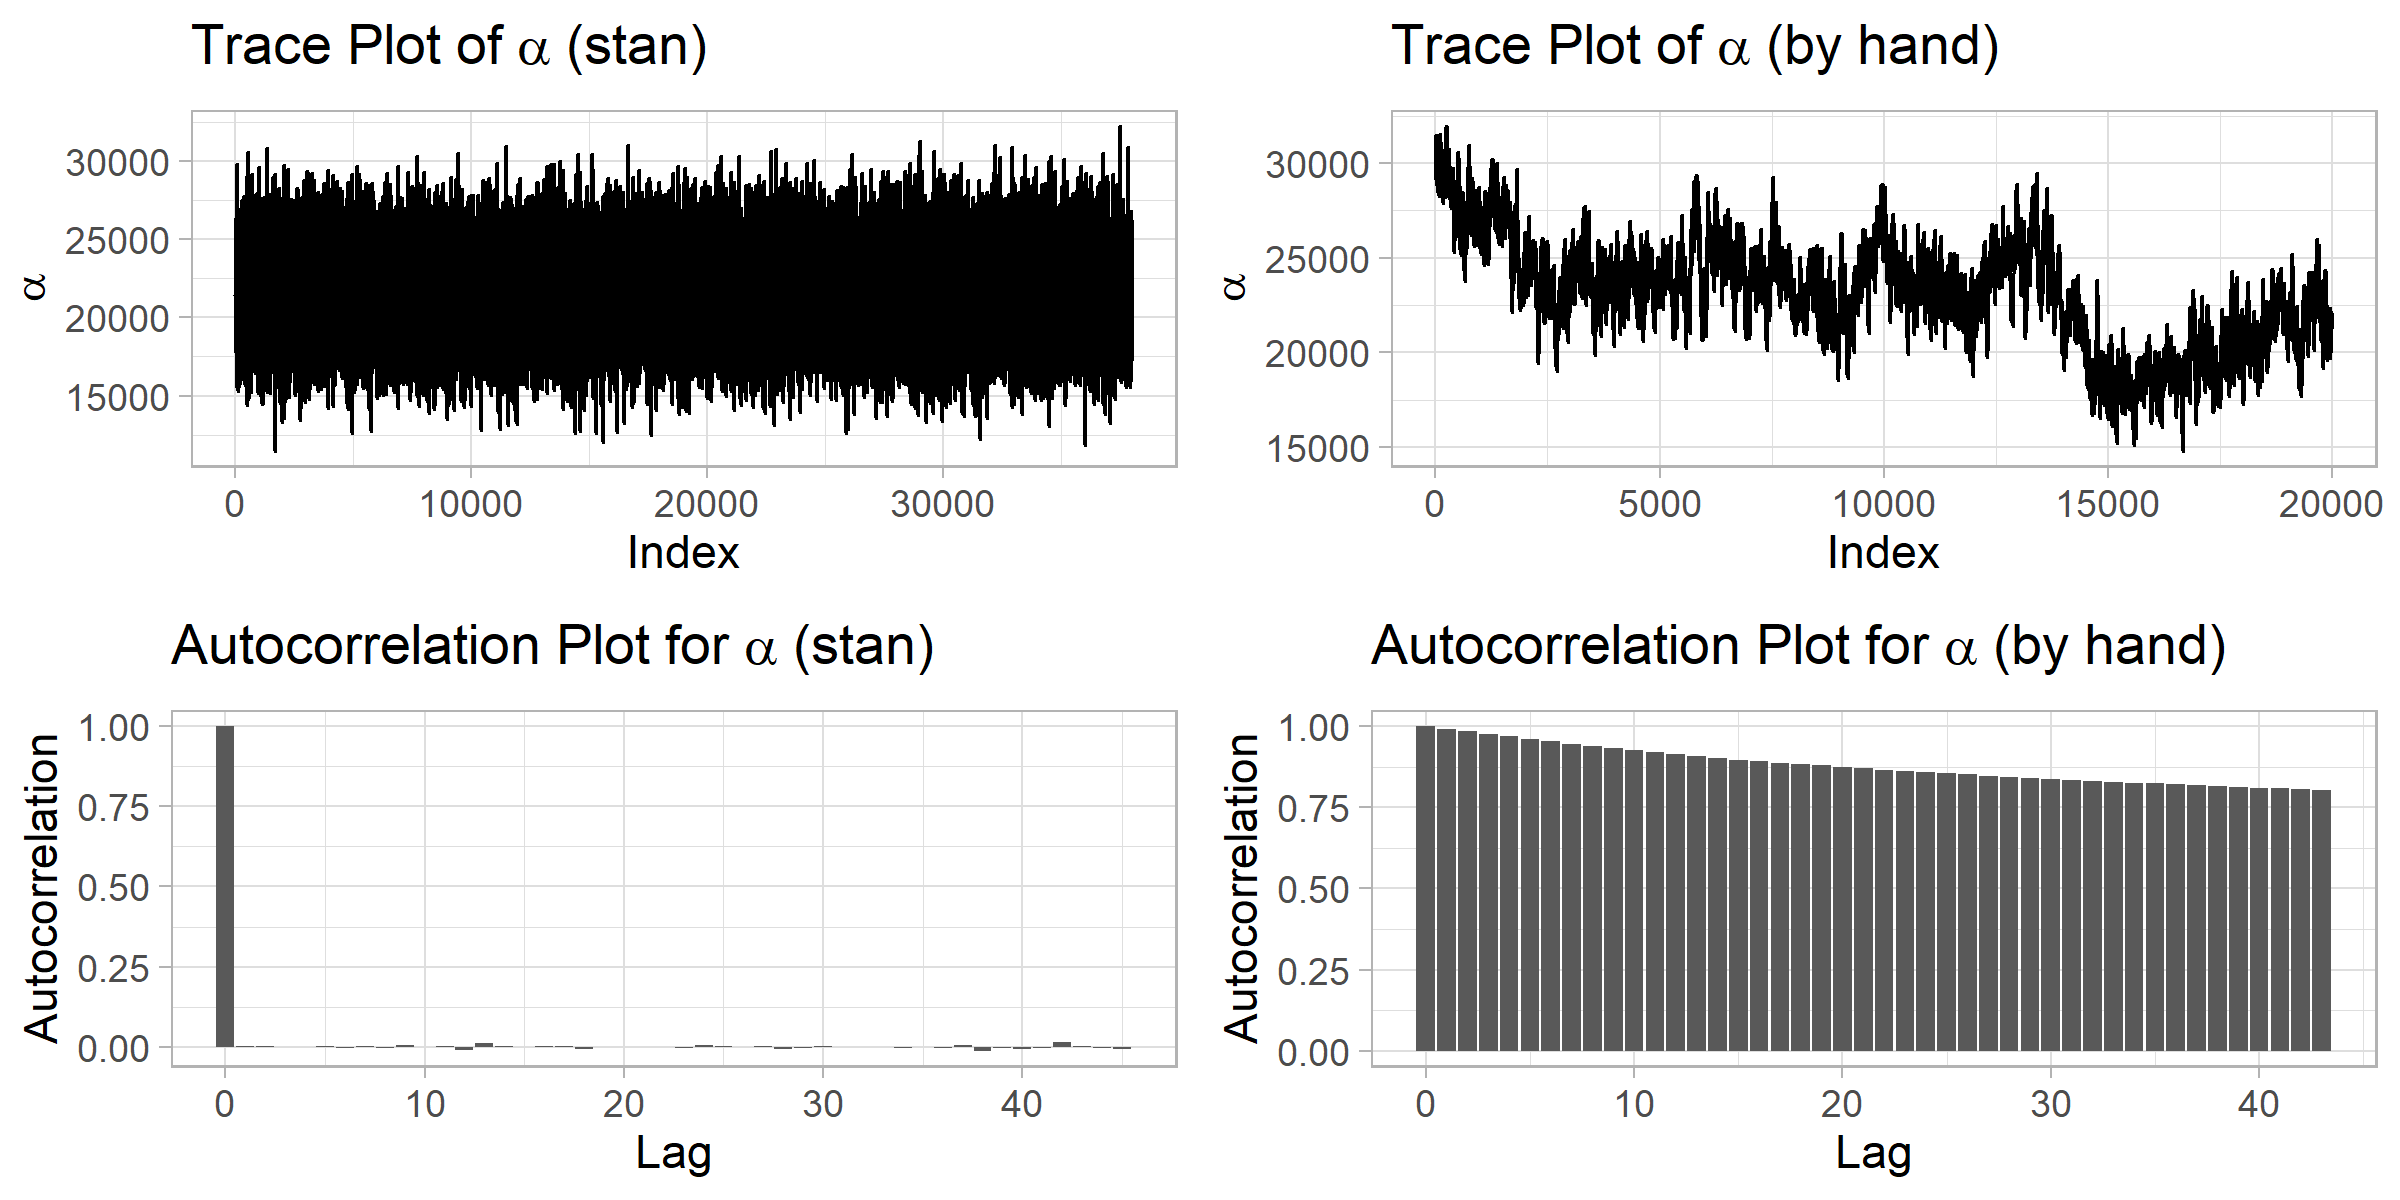
\includegraphics[width=.7\textwidth]{diagnostics.png}
    \caption{\footnotesize MCMC computational diagnostics for \code{stan} samples and by-hand samples. The trace plot for the by-hand samples reveals concerns for convergence. The ACF plot shows high autocorrelation, which would require severe thinning. The \code{stan} plots (left) show no concerning trends. These plots are only for $\alpha$, but plots for all parameters would give the same takeaways for the two sampling methods. \vspace*{-.5\baselineskip}}
    \label{fig:diagnostics}
\end{figure}

Autocorrelation plots reveal the correlation in the samples between iterations. An ideal ACF plot will have a bar of $1$ at a lag of $0$ and nearly $0$ for all other lags. If the autocorrelation remains high across the lags, then the samples are highly correlated with each other. This means that the effective sampling size would be small and estimates will have more MC error. The proper solution for high autocorrelation is thinning the samples. Figure \ref{fig:diagnostics} shows that the \code{stan} samples have an ideal ACF plot, while the by-hand samples are highly correlated, even at lag(40). 

Effective sample size takes the number of MCMC samples obtained and reduces this number according to autocorrelation within the samples. The effective sample sizes of the \code{stan} samples was $>30{,}000$ for all parameters in all three priors ($36{,}000$ for $\alpha$ each time). As expected, the effective sample sizes of the by-hand samples are not ideal, ranging from $6$ to $1{,}920$ ($48$ for $\alpha$).  

The Gelman convergence statistic $\hat{R}$ (also known as the Potential Scale Reduction Factor, PSRF) may reveal convergence issues. This metric requires at least two chains to measure mixing. Because the by-hand samples only have one chain (and the trace plots have visual evidence of convergence concerns anyway), the $\hat{R}$ metric is calculated only for the \code{stan} samples. Any $\hat{R}$ above $1.1$ is a cause for concern, and the closer to $1$, the better. If this value is too high, more samples could resolve the issue. Across all parameters and the three priors, the largest $\hat{R}$ was $1.0003$, so there is no cause for concerns about mixing with any of the parameters.

\vspace*{-.5\baselineskip}
\subsection{Frequentist Approach}

As a comparison to the Bayesian methods, an equivalent Frequentist solution was employed. This regression model has the same likelihood function as that in Equation \ref{eq:model}, so the model is as follows:
\begin{align}\label{eq:likelihood}
    y_{i,t}&\sim\mathcal{N}\left(\alpha_i+{\beta_i} * y_{i,t-1} +\theta * x_{i,t},\sigma^2\right)
\end{align}
This linear model is numerically equivalent to an ARIMA model, but with no integrated or moving average pieces and a single lag for the auto-regressive piece. One clear advantage of this model is computational burden (calculation instead of sampling). The downside is that intuitive posterior distributions are not available, and there is no possibility for a hierarchical structure or the imposition of priors. 

\vspace*{-.5\baselineskip}
\section{Results}

As shown in Section \ref{sec:diag}, the \code{stan} sampling shows no causes for concern, while the by-hand samples may not be converging correctly and have high auto-correlation. Aside from the team-specific parameter estimates, Table \ref{tab:results} shows the results from the 3 priors using \code{stan} sampling, the first prior using by-hand sampling, and the Frequentist linear model. The by-hand samples (used for the first prior) are within (or close to within) MC error for all $4$ parameters. Considering the sampling convergence issues, the assumption that the \code{stan} and by-hand samples are coming from the same posterior distribution is deemed satisfied. The remainder of this project considers only the \code{stan} samples. 

\begin{table}[ht]
    \centering
    \footnotesize
    \begin{tabular}{lccccc}
         & \code{stan} Prior 1 & By-hand (MC error) & \code{stan} Prior 2 & \code{stan} Prior 3 & LM \\
        \hline
        $\theta$ & \shortstack{$269$ \\ ($159$ to $381$)} & $272$ ($\pm4$) & \shortstack{$310$ \\ ($198$ to $422$)} & \shortstack{$297$ \\ ($187$ to $407$)} & $314$ ($\pm57$) \\
        \\
        $\alpha$ & \shortstack{$21{,}823$ \\ ($16{,}676$ to $26{,}909$)} & $22{,}440$ ($\pm378$) & \shortstack{$28{,}366$ \\ ($-8{,}630$ to $65{,}544$)} & \shortstack{$36{,}864$ \\ ($30{,}549$ to $43{,}222$)} & $30{,}460$ ($\pm4{,}353$) \\
        \\
        $\beta$ & \shortstack{$.64$ \\ ($.57$ to $.72$)} & $.63$ ($\pm.01$) & \shortstack{$.48$ \\ ($-6.12$ to $7.04$)} & \shortstack{$.51$ \\ ($.37$ to $.66$)} & $.51$ ($\pm.06$) \\
        \\
        $\sigma$ & \shortstack{$3{,}683$ \\ ($3{,}469$ to $3{,}912$)} & $3{,}678$ ($\pm3$) & \shortstack{$3{,}627$ \\ ($3{,}414$ to $3{,}854$)} & \shortstack{$3{,}635$ \\ ($3{,}427$ to $3{,}858$)} & $3{,}631$ \\
        \hline
    \end{tabular}
    \caption{\footnotesize Model Results. The Bayesian estimates under squared-error loss are shown for the \code{stan} and by-hand samples. In parentheses are the credible intervals for the \code{stan} sample parameters and the MC error for the by-hand samples. The regression estimates for the simple linear model are shown in the ``LM" column, with the standard error in parentheses. The $\alpha$ and $\beta$ estimates for LM are the mean team intercepts and effects (with standard errors).}
    \label{tab:results}
\end{table}

The team-specific results from the second prior show that the Washington Football Team (estimate of $.89$ and $95\%$ CI of $.64$ to $1.14$), Chargers (estimate of $.89$ and $95\%$ CI of $.74$ to $1.03$), and Cowboys (estimate of $.88$ and $95\%$ CI of $.75$ to $1.00$) are most influenced by prior year's attendance. The Steelers (estimate of $.01$ and $95\%$ CI of $-.68$ to $.72$), Jaguars (estimate of $.10$ and $95\%$ CI of $-.22$ to $.43$), and Panthers (estimate of $.16$ and $95\%$ CI of $-1.75$ to $2.10$) have the least evidence of being influenced by prior year's attendance. 

The Bayesian estimates under squared-error loss for team-specific intercepts and attendance effects under the three different priors are shown in Figure \ref{fig:team_spec}. The first prior restricted the possibilities, so each team is relatively similar for the team-specific effects. The second prior gave wide flexibility, so teams were allowed to deviate greatly from the overall mean (hence these results are used in the preceding paragraph). The third prior was stringent on overall effects, but the teams were also allowed to vary.

\begin{figure}
    \centering
    
\includegraphics[width=\textwidth]{team_specific.png}
    \caption{\footnotesize Estimates of team-specific intercepts and prior year's attendance effects under squared error loss. \vspace*{-.5\baselineskip}}
    \label{fig:team_spec}
\end{figure}

The final result discussed in this project is prediction for 2020. Using the posterior predictive distribution (with the Bayesian structure defined in Equation \ref{eq:model}), predictions were made for 2020 using the attendance and wins from 2019 under the first set of priors. These predictions are shown in Figure \ref{fig:preds}, including also the observed weekly average home game attendance in red. The teams that have given up the most seats are the Jets, Packers, and Giants. The teams that have given up the fewest are the Chargers, Bengals, and Buccaneers. Attendance in 2020 for the NFL is at $8\%$ of what was predicted by the Bayesian model. If revenue per seat is the same in 2020 as it was in 2019, and the average attendance doesn't change for the rest of the season from what has happened so far, the Bayesian model estimates that the NFL will have lost a staggering $\$2.11$ bil. in ticket sales alone.  

\begin{figure}
    \centering
    
\includegraphics[width=\textwidth]{Predictions.jpg}
    \caption{\footnotesize Predicted weekly attendance in 2020. The blue represents the distribution of these predictions (estimate under squared error loss represented by blue line) and the red represents the observed weekly home-game attendance so far in 2020 (according to  \href{http://www.espn.com/nfl/attendance}{ESPN.com}). \vspace*{-.5\baselineskip}}
    \label{fig:preds}
\end{figure}

%\subsection{Plots of Pooled Lines}

\vspace*{-.5\baselineskip}
\section{Conclusion}

The goals of this project were to develop a Bayesian hierarchical time series model on weekly average attendance, estimate the team-specific intercepts and prior year attendance effects along with overall effect of wins and standard error of model, and compare the results of this model to a Frequentist linear model.

A by-hand Metropolis samples was used on one set of priors and a \code{stan} Hamiltonian MCMC sampler was used on this and two other sets of priors. The results between the two approaches agreed approximately within MC error. Across the three priors, the effect of an additional win on the next year's weekly attendance is about $300$. The team-specific formula for attendance was roughly $\text{Attendance}_{t}=25{,}000 + .55\times\text{Attendance}_{t-1} + 300\times\text{Wins}_{t-1}+\epsilon,~\epsilon\sim\mathcal{N}(0,3{,}650)$, although the intercept and coefficient for prior attendance varied across teams (and priors). These results agree with those from the Frequentist linear model, but give the added benefit of hierarchical parameters and intuitive posterior distributions for the parameters. The results show that the Washington Football Team is most influenced by prior year's attendance and the Steelers have least evidence for any effect of prior year attendance. The first prior led to fairly similar team-specific intercepts and effects across teams (as per design of the prior). The second and third sets of priors led to more varying results. Predictions for 2020 show that the NFL will likely lose $>\$2$ bil. in ticket sales due to the pandemic.

One weakness of this project is the computational efficiency. Many different methods could improve the sampling efficacy in the future. For example, although the full conditional distributions are not known sampling distributions, the inverse-CDF method could be used as part of Gibb's sampling. Additionally, QR factorization of the input data could make convergence faster. Neither method was used here, because the by-hand samples matched the \code{stan} samples, which didn't have any signs of convergence issues.

There are many ways that this project could be expanded in the future. A simple method would be to make the effect of games term $\theta$ and the variance term $\sigma^2$ be team specific. Instead of modeling yearly average, the weekly attendance could be modeled as well. Other variables could also have been incorporated in such a model (e.g. weather, opposing team, prior week's performance, or other day-specific variables). Another way to improve this method would have been to model the capacity of the football stadiums. The Patriots, for example, consistently hit the maximum capacity and naively assuming no maximum capacity is a weakness of this project. Additionally, more lags, or the other elements of an ARIMA model could be employed in a Bayesian context.

\vspace*{-.5\baselineskip}
\bibliography{bib}
\bibliographystyle{agsm}


\end{document}